\section{Research Questions and Scope}\label{section:rq}

This motivated us to explore alternative ways to represent participants in WVC applications to increase engagement, interactivity, and attention. 

In distant-learning classes, for example, presenters (e.g. professors, teachers, students) often feel distracted or disengaged when there are no audiovisual feedback coming from the audience. These feedback include eye contact, gaze direction, and other body language cues.

We are set out to build a prototype WVC application to study the perceived effects of eye-contact, gaze, and head orientation in a virtual 3D space to make up the missing aspects from in-person F2F interactions.

Our project explores whether adding eye-contact to the current WVC system will enhance the sense of interaction and presence of the users. Conventional WVC services only offer standard visual and audio communication, and they do not support intuitive and personalized eye-contact between users. Therefore, people still prefer face-to-face meetings because of the highly interactive meeting environment.

We propose FutureGazer, a WVC system that simulates eye-contact and gaze amongst the participants in a WVC meeting room to enable a highly interactive environment. Our project explores whether adding eye-contact to the current WVC system will enhance the sense of interaction and presence of the users. Conventional WVC services only offer standard visual and audio communication, and they do not support intuitive and personalized eye-contact between users. Therefore, people still prefer face-to-face meetings because of the highly interactive meeting environment\cite{rn42}.

To test our system, we recruit friends and students are participants to study the effects of the additional eye contact and gaze cues in online meeting environments. Figure \ref{fig:intro-a} shows what we intend to build in contrast to existing WVC platforms like Zoom. Figure \ref{fig:intro-b} depicts the personalized eye-contact simulation enabled by our system.

\begin{figure}
	\centering
 	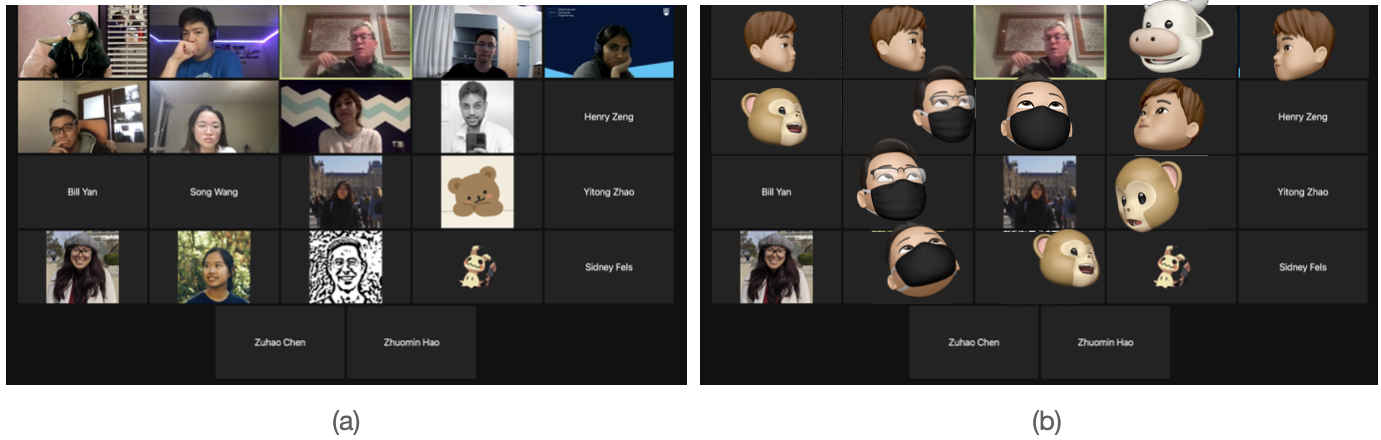
\includegraphics[width=0.9\textwidth]{introA.png}
	\caption{(a) Current WVC model: each participant stays in their grid and no eye contact interaction. (b) Proposed model: students can look at each other to create virtual eye-contact.}
	\label{fig:intro-a}
\end{figure}

\begin{figure}
	\centering
 	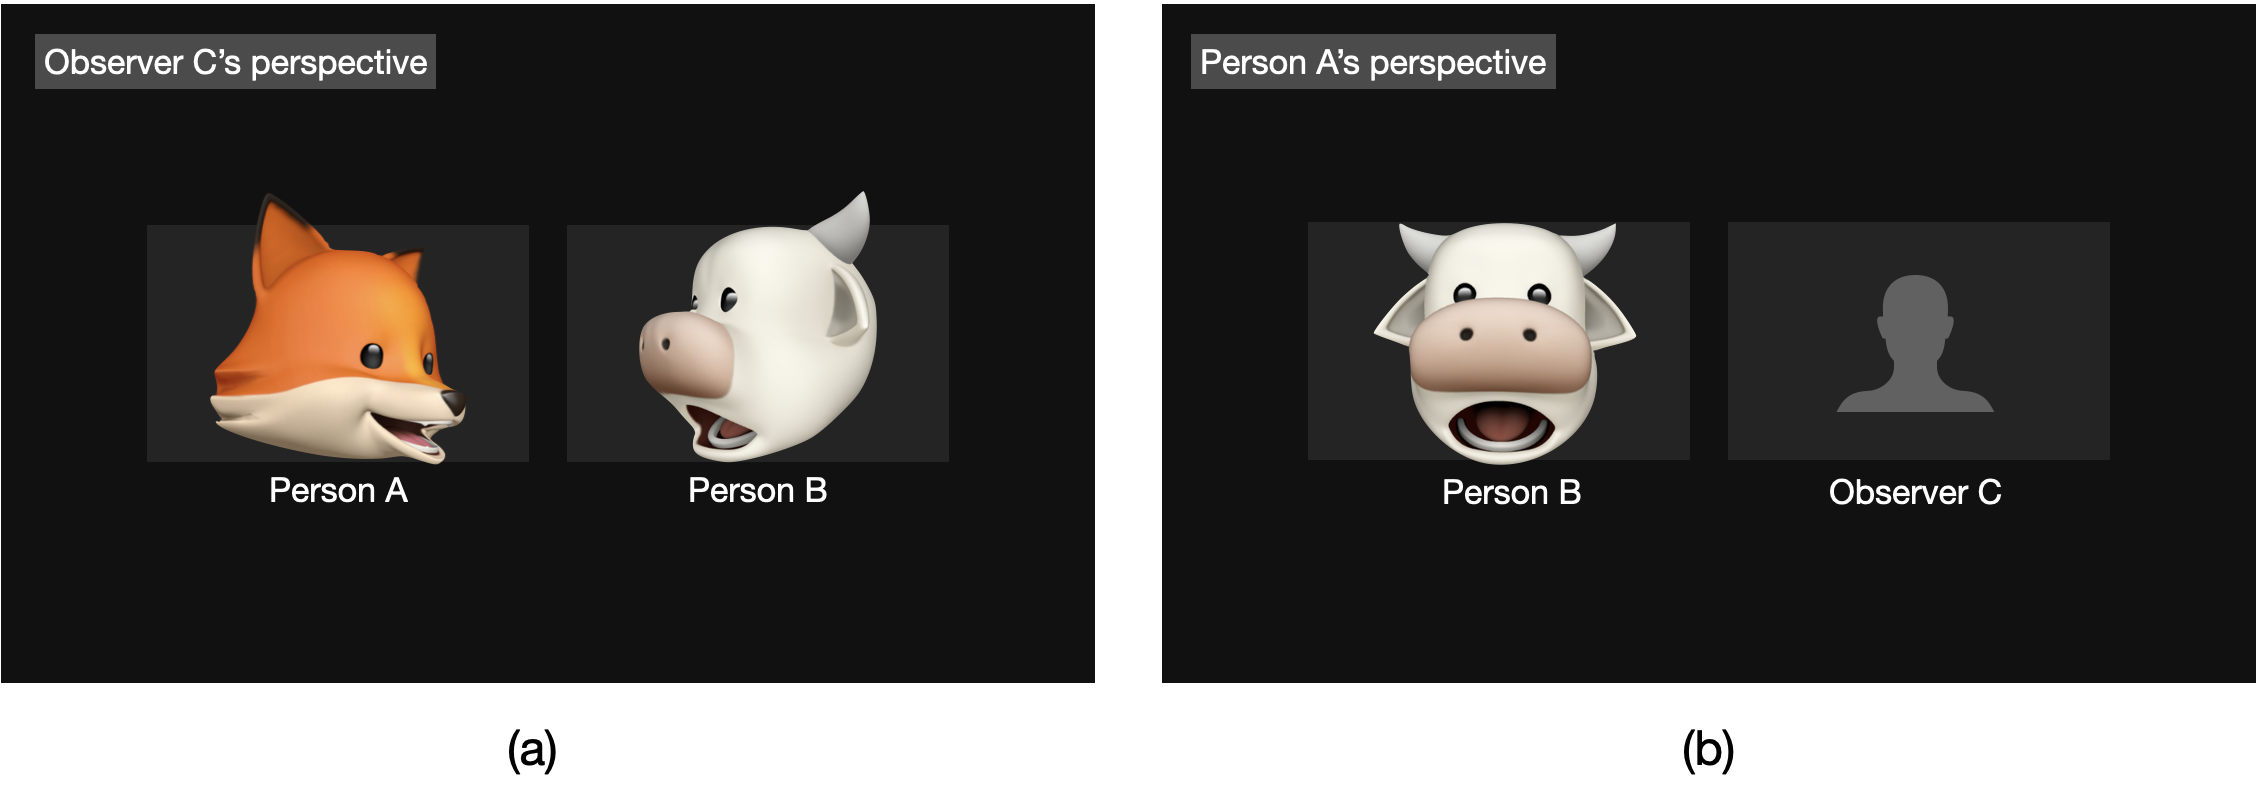
\includegraphics[width=0.9\textwidth]{introB.png}
	\caption{(a) Observer’s perspective in a meeting room with person A (fox) and person B (cow) looking at each other. (b) Person A’s perspective in the exact same meeting room at the exact same time.}
	\label{fig:intro-b}
\end{figure}

The key metrics we want to observe in this project are: participant’s attention, engagement, and the feeling of connectedness. To explore parameters that effect these metrics, we consolidate these ideas into three core research questions (hereafter will be refer to as \textbf{RQ1}, \textbf{RQ2}, and \textbf{RQ3}):

\begin{enumerate}
    \item Can a person tell if they are being looked at in a WVC and how can 3D avatars be augmented to enhance this experience.
    \item Can a person tell if other participants are looking at each other in a WVC and how using 3D avatars can be augmented to increase engagement.
    \item How does a person’s attention change as the avatars augmented with WVC enables eye-contact and gaze.
\end{enumerate}

